%
% File naaclhlt2010.tex
%
% Contact: nasmith@cs.cmu.edu

\documentclass[11pt,letterpaper]{article}
\usepackage{naaclhlt2010}
\usepackage{times}
\usepackage{latexsym}
\usepackage{amsmath}
\usepackage{graphicx}
\graphicspath{ {pic/} } 
\setlength\titlebox{6.5cm}    % Expanding the titlebox

\title{CS475 Final Project\\Neural Network for Handwritten Digits Recognition}

\author{Li-Yi Lin\\
  Computer Science, JHU\\
  {\tt llin34@jhu.edu}
  \And
  Chenyang Su \\
  Mathematics, JHU\\
  {\tt csu8@jhu.edu}}

\date{}

\begin{document}
\maketitle
\begin{abstract}
Neural network has been successfully applied to many machine learning topics such as speech and object recognitions, and machine translation in recent years. Neural network can learn new features automatically instead of doing feature engineering by hand, making it very powerful of dealing with complex problems.
          
In this project, we implemented and applied neural network techniques to do handwritten digits recognition. The shapes of handwritten digits varies from people to people, thus are difficult for simple machine learning algorithms to classify them. We investigated how to apply neural network to this recognition problem and got hands-on experience by implementing the algorithm and tuning parameters. Finally we compared our result with that from applying external SVM library and explained some possible factors that can affect the performance of the learning algorithms.
\end{abstract}

\section{Introduction}

Human handwriting recognition is an interesting problem with various applications. In our project we focus on handwritten digits recognition, which has already been extensively studied before. Our dataset is the famous “Modified National Institute of Standards and Technology (MNIST)” dataset downloaded from Kaggle\footnote{https://www.kaggle.com/c/digit-recognizer/data}. The data has already been preprocessed and stored into csv formats. Every image in the MNIST dataset is 28 pixels in width and 28 pixels in height. So every instance in the training data files has 784 features corresponding to the 784 pixels. The value of each feature is 0-255 to indicate the darkness of the pixel. The training dataset also contains a label column indicating the digits 0-9. Therefore this is a supervised learning problem. 

This problem is clearly nonlinear, and has a large amount of features, making it hard for  applying simple linear classification algorithm. To solve this complex problem, neural network can transform linear combination of original features nonlinearly into new useful features. 

Neural network is inspired by the human’s central nervous systems. Each node represents the neuron in the brain system and is connected together to form a neural network.  The similarity in structure as the human brain makes the neural network a powerful tool to give accurate predictions in complicated problems. 



\section{Description of Methods}
\subsection{Neural Network}

A neural network consists of several layers, where the first layer is the input layer, the last layer is the output layer and all the other layers are called hidden layers. Each layer has several nodes and there are edges connecting nodes in neighboring layers. See figure \ref{neural network}.

In a neural network, the $l-th$ layer contains $d^{(l)}+1$ nodes $x_0^{(l)},x_1^{(l)},x_2^{(l)},...,x_{d^{(l)}}^{(l)}$, where $x_0^{(l)}$ is always the bias term constant 1. $x_j^{(l)}$ is calculated by passing the linear combination of all $x_i^{(l-1)}$ to a nonlinear activation function $\theta$, which in our problem is the sigmoid function $\theta(z)=\frac{1}{1+e^{-z}}$. Mathematically,
$$x_j^{(l)}=\theta(s_j^{(l)})=\theta\left(\sum_{i=0}^{d^{(l-1)}}w_{ij}^{(l)}x_i^{(l-1)}\right)$$,
where $s_j^{(l)}=\sum_{i=0}^{d^{(l-1)}}w_{ij}^{(l)}x_i^{(l-1)}$ is called the signal. Starting from the input layer, we apply the above formula to get all the nodes in the first hidden layer. Then repeating the process to each hidden layer one by one, we get all the hidden nodes and finally get the nodes in output layer. Output layer contains nodes corresponding to labels (in handwritten digits problem we have 10 labels). We will predict the label with the largest output value. The above procedure is the feed forward step in neural network. 

Therefore the accuracy of prediction depends on $w_{ij}^{(l)}$, which are the parameters we need to learn. In neural network, the learning step is done by back propagation. We first denote $\{w_{ij}^{(l)}\}$ by $w$ and the cost by $e(w)$. According to stochastic gradient descent (SGD), we shall update $w_{ij}^{(l)}\gets w_{ij}^{(l)}-\eta\frac{\partial e(w)}{\partial w_{ij}^{(l)}}$. Applying chain rule, we have
$$\frac{\partial e(w)}{\partial w_{ij}^{(l)}}=\frac{\partial e(w)}{\partial s_j^{(l)}}\frac{\partial s_j^{(l)}}{\partial w_{ij}^{(l)}}.$$
Here it is easy to see that $\frac{\partial s_j^{(l)}}{\partial w_{ij}^{(l)}}=x_i^{(l-1)}$ and we denote $\frac{\partial e(w)}{\partial s_j^{(l)}}$ by $\delta_j^{(l)}$. $x_i^{(l-1)}$ is already calculated by feed forward. We just need to calculate $\delta_j^{(l)}$ by back propagation. We shall first give the cost function used in our problem. In the final layer $L$, which is the output layer, we have 10 nodes $x_0^{(L)},x_1^{(L)},...,x_{9}^{(L)}$. And we transform the label into a vector $(y_0,y_1,...,y_{9})$, where $y_i$ equals 1 if the label is $i$ and 0 otherwise. Then our cost function is defined as 
$$e(w)=\frac{1}{2}\sum_{i=0}^{9}(x_i^{(L)}-y_i)^2.$$

Since $x_i^{(L)}=\theta(s_i^{(L)})$, $\delta_{i}^{(L)}=\frac{\partial e(w)}{\partial s_i^{(L)}}=(\theta(s_i^{(L)})-y_i)\theta'(s_i^{(L)})$. We shall note $\theta(z)=\frac{1}{1+e^{-z}}$. Therefore $\theta'(z)=(1-\theta(z))\theta(z)$. Then $\delta_{i}^{(L)}=(x_i^{(L)}-y_i)(1-x_i^{(L)})x_i^{(L)}$. Above all we can compute $\delta$ for the final layer. To compute $\delta$ for other layers, we can apply chain rule,
\begin{align*}
\delta_i^{(l-1)}&=\frac{\partial e(w)}{\partial s_i^{(l-1)}}\\
&=\sum_{j=1}^{d^{(l)}}\frac{\partial e(w)}{\partial s_j^{(l)}}\frac{\partial s_j^{(l)}}{\partial x_i^{(l-1)}}\frac{\partial x_i^{(l-1)}}{\partial s_i^{(l-1)}}\\
&=\sum_{j=1}^{d^{(l)}}\delta_j^{(l)}w_{ij}^{(l)}\theta'(s_i^{(l-1)})\\
&=\sum_{j=1}^{d^{(l)}}\delta_j^{(l)}w_{ij}^{(l)}(1-\theta(s_i^{(l-1)}))\theta(s_i^{(l-1)})\\
&=(1-x_i^{(l-1)})x_i^{(l-1)}\sum_{j=1}^{d^{(l)}}\delta_j^{(l)}w_{ij}^{(l)}
\end{align*}  
The formula above shows how we get $\delta$ in one layer from the layer after, which is the back propagation algorithm. 

\subsection{Support vector machine (SVM)}

The method of SVM classifies data by drawing a hyperplane in space. Points in one side is classified as 0 and in another side is classified as 1. Therefore it is a linear classifier. 

However, SVM with kernel method can work well with data which are not linearly separable. Kernel method can transform the feature and produce nonlinear decision boundary.  

\begin{center}%\label{neural network}
\begin{figure*}
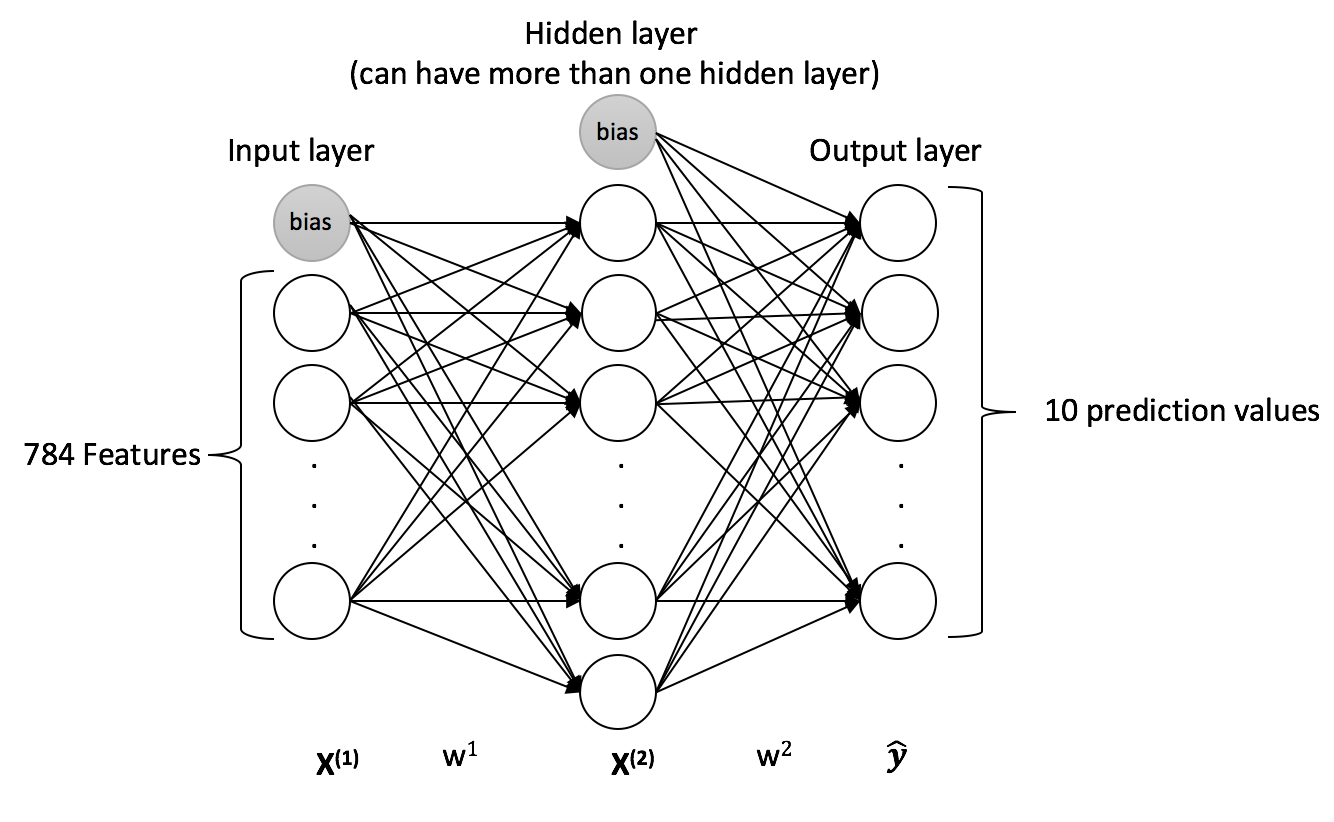
\includegraphics[scale=0.7]{net}
    \caption{Neural network}
      \label{neural network}

\end{figure*}
\end{center}
% \caption{Neural network}

\begin{center}
\begin{figure}
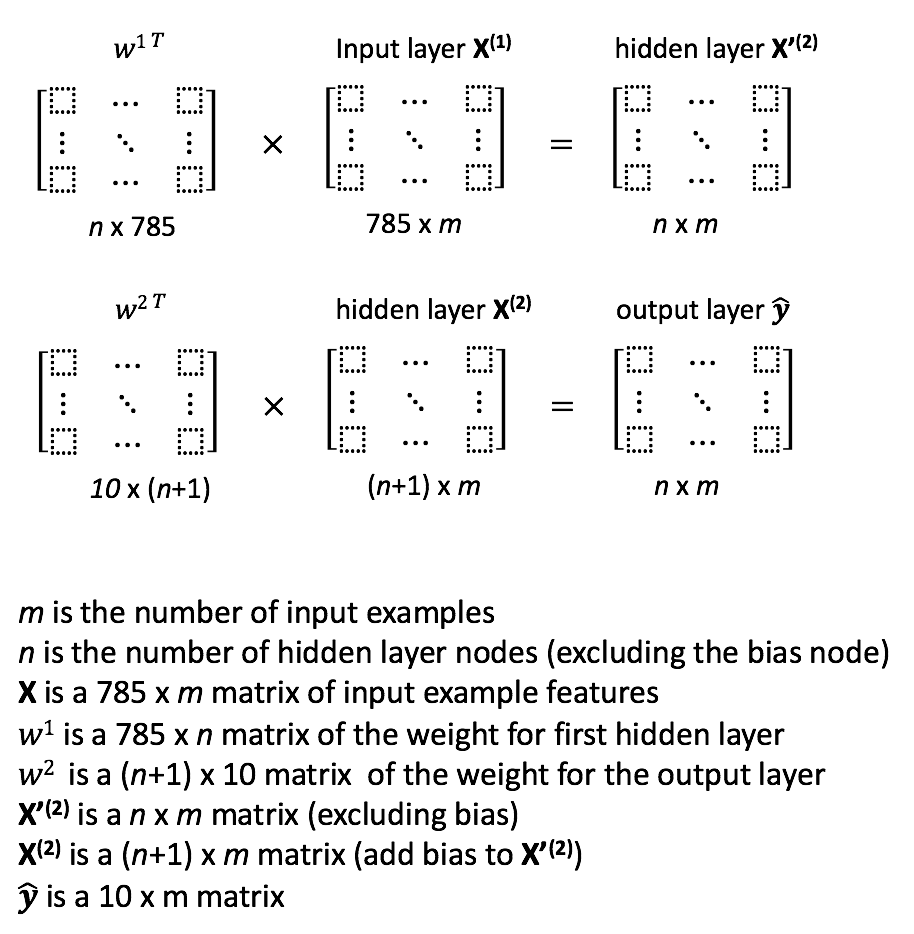
\includegraphics[scale=0.5]{matrix}
    \caption{Matrices representation}
      \label{matrices}
\end{figure}
\end{center}

\begin{center}
\begin{figure*}
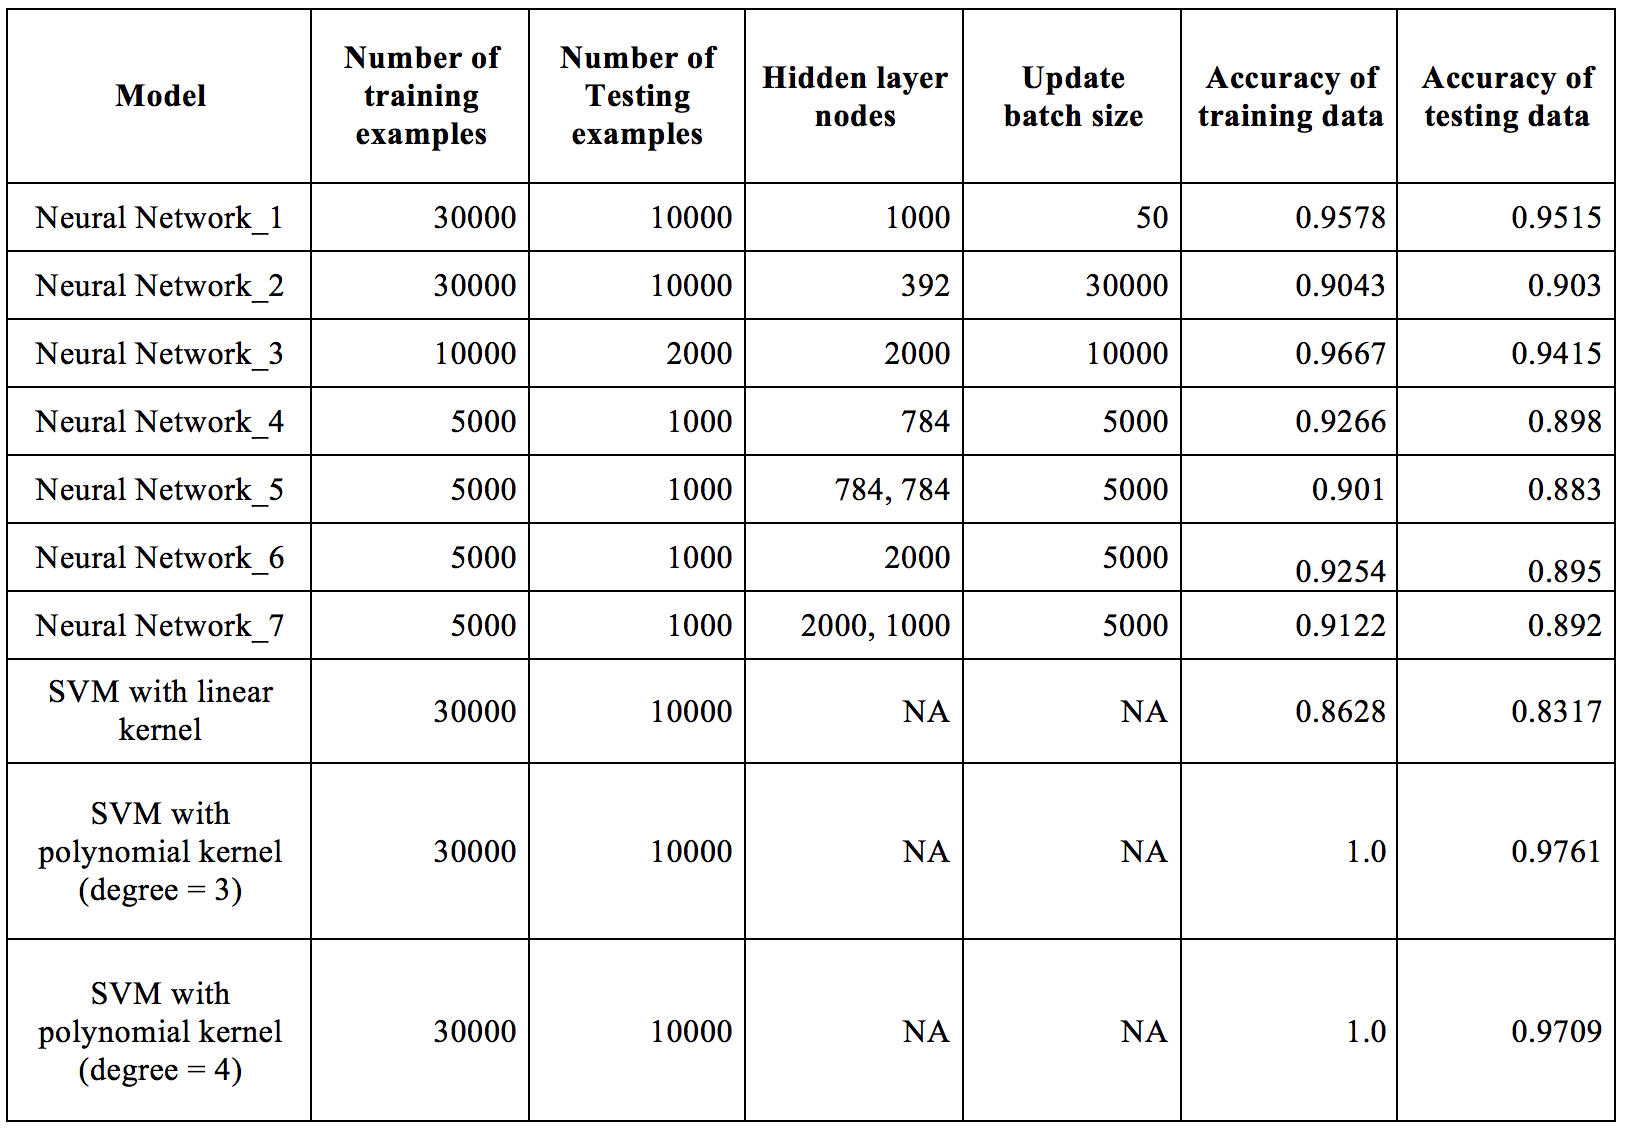
\includegraphics[scale=0.55]{table}
    \caption{Experiment results}
      \label{results}
\end{figure*}
\end{center}

\begin{center}
\begin{figure*}
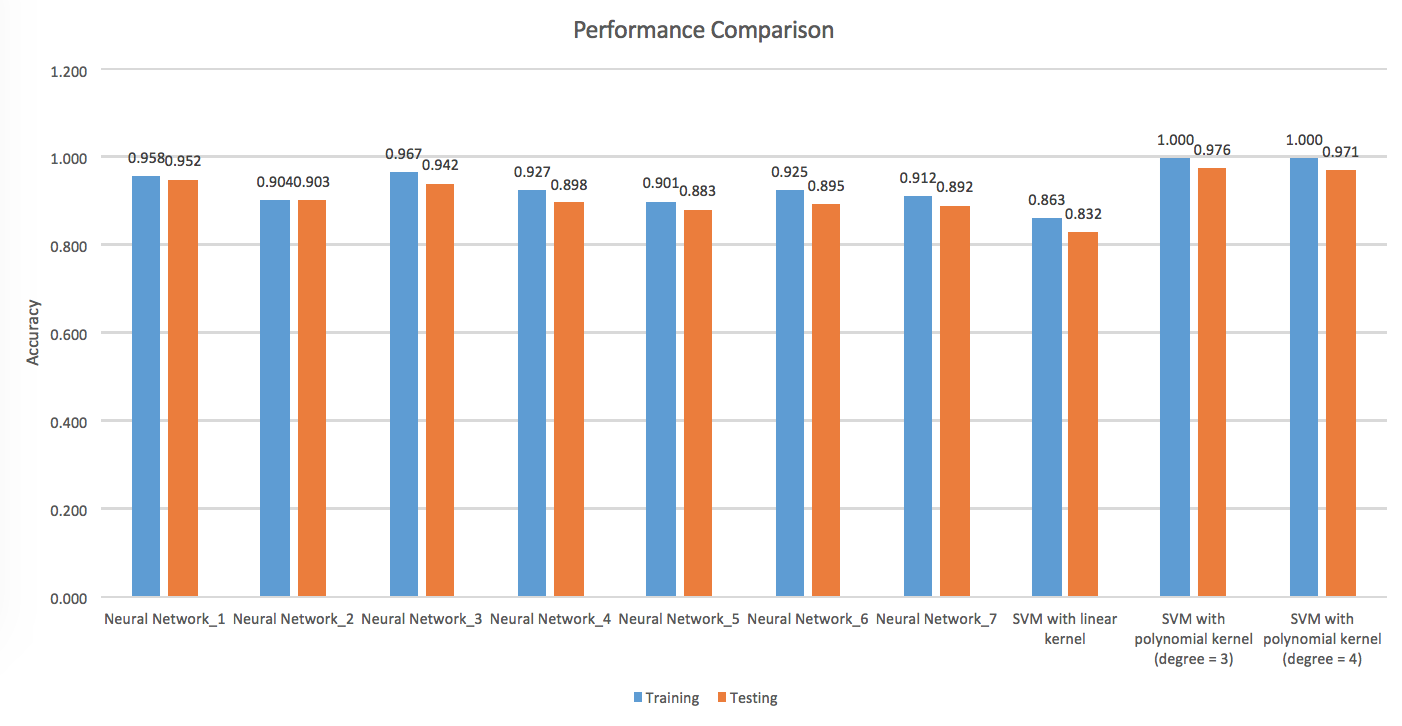
\includegraphics[scale=0.7]{models}
    \caption{Performance Comparison}
      \label{performance}
\end{figure*}
\end{center}

\begin{center}
\begin{figure*}
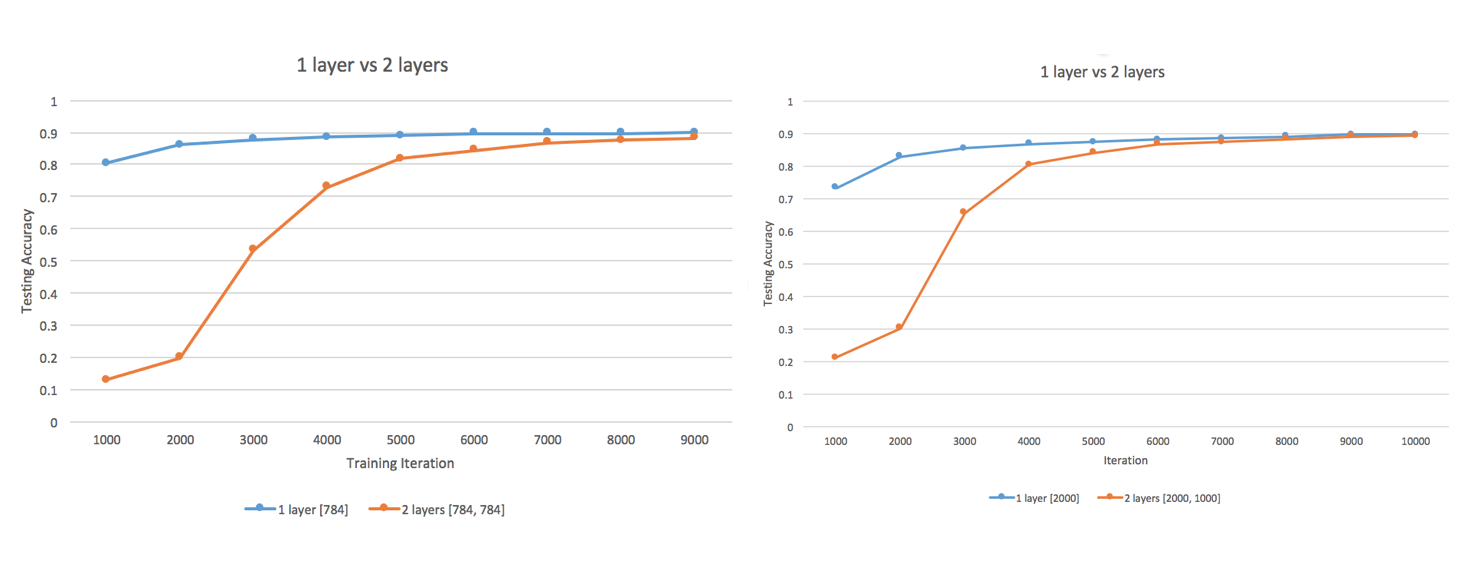
\includegraphics[scale=0.68]{layer_3}
    \caption{1 layer vs 2 layers}
      \label{12layer}
\end{figure*}
\end{center}

\section{Implementation Description}
For implementing the neural network for this project, the programming language we used is Python with NumPy (a Matlab-like library for Python). We first wrote a data loader that can load specified number of examples from a particular example index. The data loader allows us to separate the training data and testing data for specific number of examples from the “train.csv” file containing true labels for each example. While loading the data, we also performed feature scaling by dividing each feature value by 255, which is the range of each feature value. The feature scaling is an important step if we want to train the model using large number of training examples for each training iteration instead of mini-batch method. When using large number of training examples for each training iteration, it is easy to have the overflow problem if we do not apply the feature scaling pre-processing. 

After the data loader has loaded the training and testing examples and outputted them as matrices using NumPy,  we will start to train the neural network. In the beginning of the training process, we will initialize every weight matrices according to the node number in the previous layer (e.g. the previous layer for $w_1$ is the input layer). The initial weights for each element in the weight matrix are randomly generated within the interval [$-\frac{1}{nodes}, \frac{1}{nodes}$], where “nodes” indicates the number of nodes in previous layer. The neural network we implemented can have arbitrary number of hidden layers, which can also have arbitrary number of hidden nodes (the number of nodes should be at least one). In this way, we can experiment different kind of settings of the hidden layers to see the difference of the results from different neural network structures.

After initializing the weights, the neural network will perform the feedforward and backpropagation training process. Before running the training process for many iterations, we will first check whether the cost is steadily reduced in 5 iterations to make sure that we pick an appropriate learning rate. The learning rate must not make the gradient descent oscillate due to the big step size for updating the weights. For mini-batch method, the cost will not necessarily be reduced in each iteration, but should decrease in large scale. 

In the feedforward process, the program (the neural network we implemented) will produce the sigmoid value for each of the ten classes by computing the multiplication of input layer and the first weight matrix and so on to the output layer. Then the backpropagation will be performed to calculate the delta for each layer and the derivation for each weight matrix. When updating the weight matrices, we also implemented the momentum method that can accelerate the converge speed. The momentum method takes the previous update into account and multiply it with a decay factor called momentum factor. In our training process, we set the momentum factor to 0.8. In sum, the weight will be updated using the following equation: $w^{(l)} = w^{(l)} - \alpha \times (x^{(l)} \delta^{(l+1)}) + \mathrm{momentum\_factor} \times \mathrm{last\_momentum}$
% weight_i = weight_i - learning_rate * (activation_matrix_of_layer_i * delta_of_layer_i+1) + momentum_factor * last_momentum

The most difficult part of the feedforward and backpropagation is that we transform the equation into a matrix-based way so that we can utilize the power of matrix manipulation to do massive computation task. See Figure \ref{matrices}. The use of matrix is very important because the feature number is very large and if we use many training examples, the training process will take a lot of time. 

During the training process, we also output the accuracy of training data and testing data every 1000 iterations. If we see the accuracy for testing data is not getting improved or improved very slowly, the training process will be terminated.

For comparison purpose, we applied SVM classifier from sci-kit learn library, which is a well-known machine learning library for Python. The kernel we used for SVM is linear and polynomial kernel. Other parameters for the SVM will be adjust automatically by the implementation of the library.


\section{Result}
We trained the neural network using batch and mini-batch update at each iteration. We also examined different combinations of hidden layers and hidden nodes. We applied the SVM classifier with linear and polynomial kernels on the same data sets for the purpose of performance comparison. The result is shown in the following Figure \ref{results}. 

During the training process, we found that it is more likely to go into the local optimal using all the training examples for update at each iteration. If we use mini-batch, which used 50 examples for one iteration, it will not be stuck in the local optimal. We also found that the starting accuracy of two-hidden-layer neural networks will be much lower than that of one-hidden-layer neural network. See Figure \ref{12layer} However, they will eventually converge to similar accuracies. The reason we can think of is because that two layers have more parameters to be trained. So it takes more iterations to reach the converged result. Due to the limitation of time, we cannot see the impact from different hidden nodes in few experiments.

Since our problem is non-linear, the non-linear SVM has a better performance than the linear one.

% \begin{center}
% \begin{figure*}
% 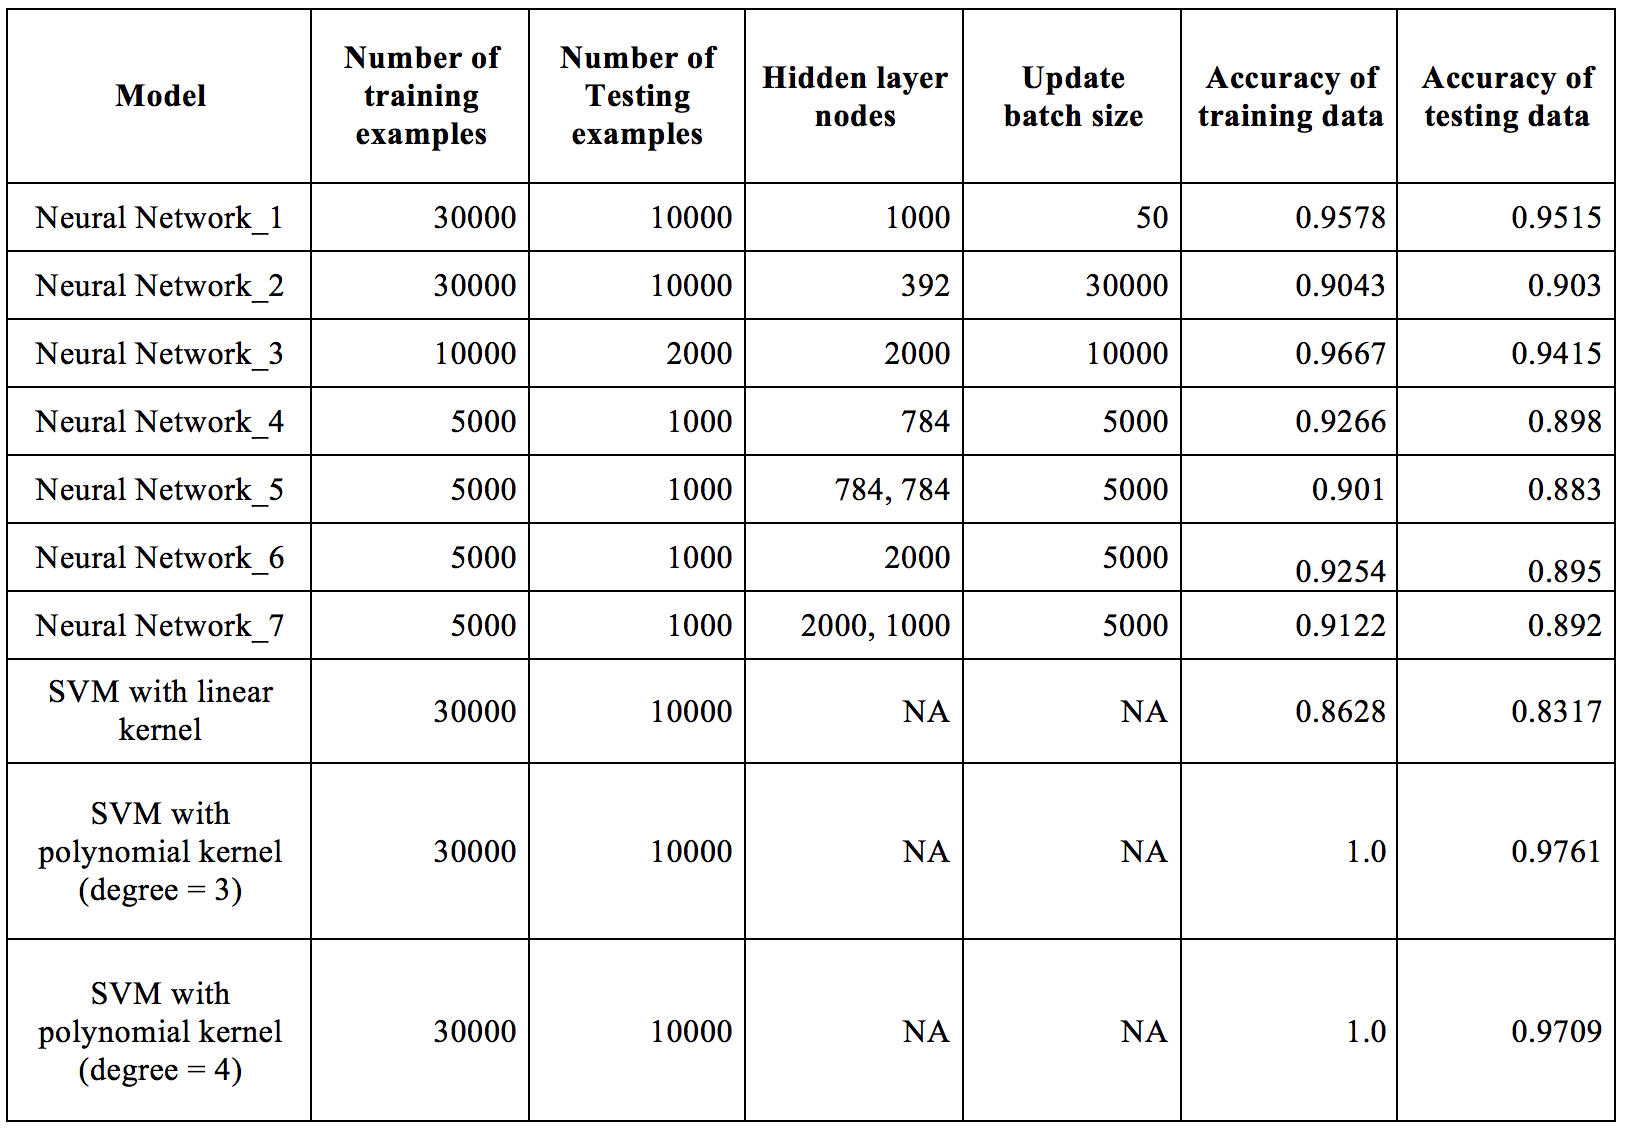
\includegraphics[scale=0.55]{table}
%     \caption{Experiment results}
%       \label{results}
% \end{figure*}
% \end{center}

% \begin{center}
% \begin{figure*}
% 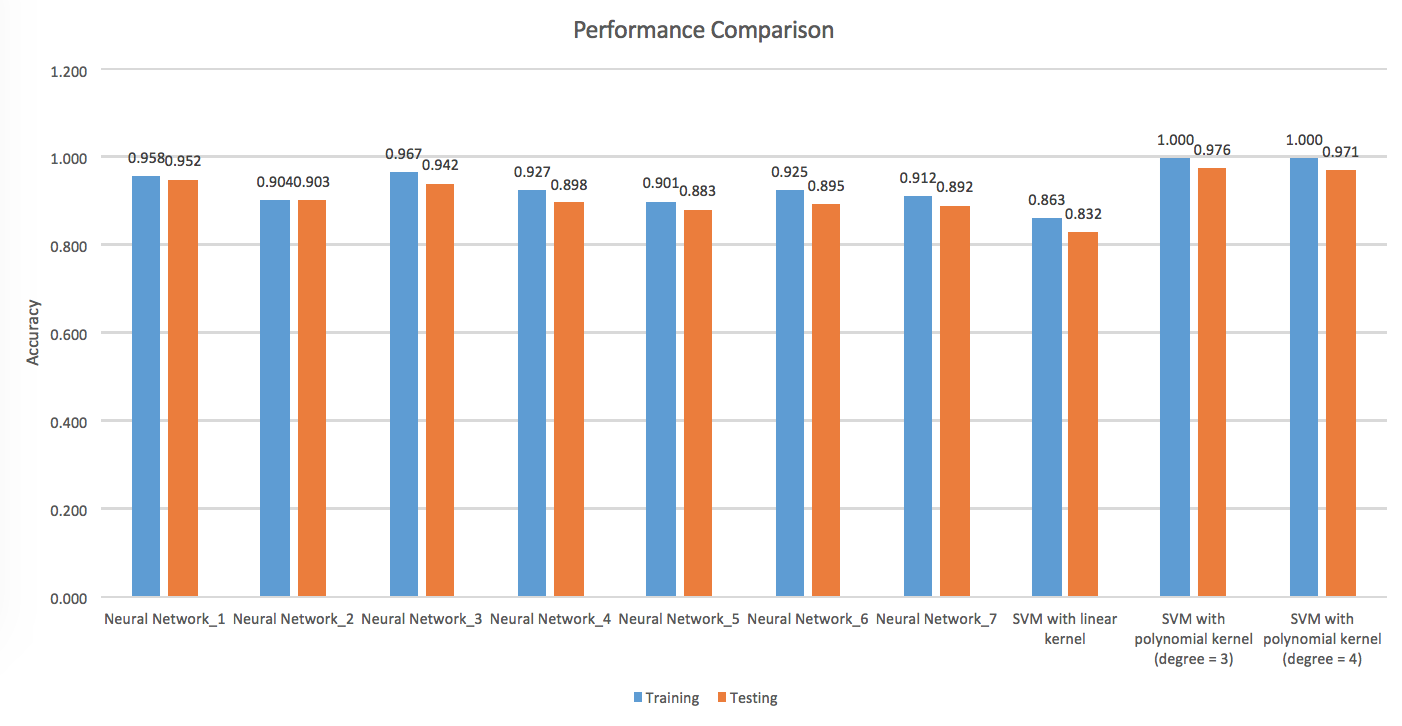
\includegraphics[scale=0.7]{models}
%     \caption{Performance Comparison}
%       \label{performance}
% \end{figure*}
% \end{center}

% \begin{center}
% \begin{figure*}
% 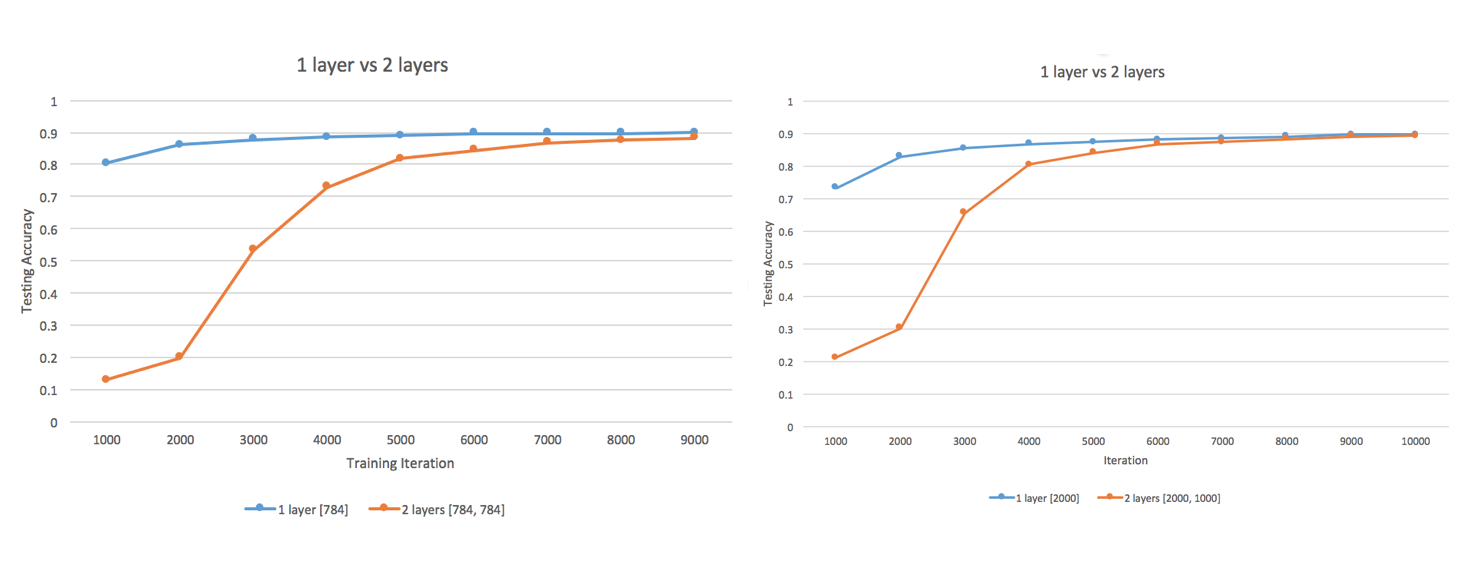
\includegraphics[scale=0.68]{layer_3}
%     \caption{1 layer vs 2 layers}
%       \label{12layer}
% \end{figure*}
% \end{center}


\section{Comparison to Proposal}
We finished the "Must achieve", "Expected to achieve", and "Would like to achieve" parts described in our proposal. For the "Must achieve" part, we fully implemented our own neural network which supports multi-hidden layer containing arbitrary hidden nodes, and batch/mini-batch update method. We also applied SVM classifier from sci-kit learn library to get results for performance comparison. For "Expected to achieve", we tuned the parameters, such as hidden layers, hidden nodes, learning rate, and batch-update size for our neural network. And the finally, the results got from our neural network is comparable to the external library. For "Would like to achieve", we gave analysis to the results for both neural network and SVM and get good understanding about how thees two algorithms work in the real world problems.

\section{References}

\begin{enumerate}
\item Stefan Knerr, LCon Personnaz, and GCrard Dreyfus, "Handwritten Digit Recognition by Neural Networks with Single-Layer Training," IEEE.
\item Chris Bishop, "Pattern Recognition and Machine Learning," 2006, Chapter 5.
\item Sci-kit learn library, http://scikit-learn.org/stable/index.html
\item Caltech online machine learning course, "Lecture 10-Neural Networks."
\end{enumerate}
% \begin{thebibliography}{}

% \bibitem[\protect\citename{Stefan Knerr, LCon Personnaz, and GCrard Dreyfus]{Ste:}
% Stefan Knerr, LCon Personnaz, and GCrard Dreyfus.
% \newblock {\em Handwritten Digit Recognition by Neural Network with Single Layer Training.},
% \newblock IEEE.

% \bibitem[\protect\citename{{American Psychological Association}}1983]{APA:83}
% {American Psychological Association}.
% \newblock 1983.
% \newblock {\em Publications Manual}.
% \newblock American Psychological Association, Washington, DC.

% \bibitem[\protect\citename{{Association for Computing Machinery}}1983]{ACM:83}
% {Association for Computing Machinery}.
% \newblock 1983.
% \newblock {\em Computing Reviews}, 24(11):503--512.

% \bibitem[\protect\citename{Chandra \bgroup et al.\egroup }1981]{Chandra:81}
% Ashok~K. Chandra, Dexter~C. Kozen, and Larry~J. Stockmeyer.
% \newblock 1981.
% \newblock Alternation.
% \newblock {\em Journal of the Association for Computing Machinery},
%   28(1):114--133.

% \bibitem[\protect\citename{Gusfield}1997]{Gusfield:97}
% Dan Gusfield.
% \newblock 1997.
% \newblock {\em Algorithms on Strings, Trees and Sequences}.
% \newblock Cambridge University Press, Cambridge, UK.

% \end{thebibliography}

\end{document}
